\documentclass[12pt,a4paper]{article}

% ==========================================================
% CONFIGURACIÓN GENERAL
% ==========================================================
\usepackage[utf8]{inputenc}
\usepackage[T1]{fontenc}
\usepackage[spanish]{babel}

\usepackage[
 a4paper,
 top=2.5cm,
 bottom=2.5cm,
 left=3cm,
 right=3cm,
 headheight=70pt
]{geometry}

% ==========================================================
% PAQUETES
% ==========================================================
\usepackage{lmodern}
\usepackage{amsmath}
\usepackage{amssymb}
\usepackage{graphicx}
\usepackage{xcolor}
\usepackage{float}
\usepackage{booktabs}
\usepackage{tabularx}
\usepackage{array}
\usepackage{enumitem}
\usepackage{multicol}
\usepackage{subcaption}
\usepackage{fancyhdr}
\usepackage{listings}
\usepackage{hyperref}
\usepackage{microtype}
\usepackage{longtable}

% Color utilizado en las listas
\definecolor{accentblue}{RGB}{31,78,121}

% ==========================================================
% CONFIGURACIÓN DE HYPERREF
% ==========================================================

\hypersetup{
 colorlinks=true,
 linkcolor=black,
 filecolor=black,
 urlcolor=blue,
 citecolor=black,
 pdftitle={Sistema Difuso MIMO y Algoritmos Geneticos para Semaforizacion Inteligente},
 pdfauthor={Marlon Guevara}
}

% ==========================================================
% COMANDO PARA CHECKBOX
% ==========================================================

\newcommand{\checkedbox}{\boxtimes}

% ==========================================================
% ENCABEZADO Y PIE DE PÁGINA
% ==========================================================

\pagestyle{fancy}

\fancyhf{}

\fancyhead[C]{%
 \begin{minipage}[c]{2.5cm}
 \centering
 \textbf{\includegraphics[width=1.2cm]{imagenes/uta.png}}
 \end{minipage}%
 \hfill
 \begin{minipage}[c]{8cm}
 \centering
 \small \textbf{UNIVERSIDAD TÉCNICA DE AMBATO}\\[0.1cm]
 \scriptsize \textit{
 FACULTAD DE INGENIERÍA EN SISTEMAS,
 ELECTRÓNICA E INDUSTRIAL}\\[0.1cm]
 \scriptsize \textbf{CARRERA DE SOFTWARE}\\[0.1cm]
 \scriptsize \textbf{CICLO ACADÉMICO: AGOSTO -- DICIEMBRE 2026}
 \end{minipage}%
 \hfill
 \begin{minipage}[c]{2.5cm}
 \centering
 \textbf{\includegraphics[width=1.2cm]{imagenes/fisei.png}}
 \end{minipage}%
}

\fancyfoot[C]{\thepage}

% ==========================================================
% INICIO DEL DOCUMENTO
% ==========================================================

\begin{document}

% ==========================================================
% PORTADA (se conserva la estructura del documento original)
% ==========================================================

\begin{center}

\vspace*{1cm}

{\Large \textbf{UNIVERSIDAD TÉCNICA DE AMBATO}}

\vspace{0.3cm}

{\large
\textbf{FACULTAD DE INGENIERÍA EN SISTEMAS,
ELECTRÓNICA E INDUSTRIAL}}

\vspace{0.3cm}

{\large \textbf{CARRERA DE SOFTWARE}}

\vspace{1.5cm}

\textbf{\includegraphics[width=4cm]{imagenes/uta.png}}

\vspace{1.2cm}

{\Large \textbf{PROYECTO DE INTELIGENCIA ARTIFICIAL}}

\vspace{1cm}

{\large
\textbf{Optimización Ambiental de la Semaforización Urbana mediante un
Sistema de Inferencia Difusa Multivariable (MIMO), Algoritmos Genéticos
y Extracción de Reglas con el Algoritmo PRISM}}

\vspace{1.5cm}

\begin{flushleft}

\textbf{Unidad de Organización Curricular:}
Profesional

\vspace{0.2cm}

\textbf{Asignatura:}
Inteligencia Artificial

\vspace{0.5cm}

\textbf{Alumno participante:}

\begin{itemize}
 \item Guevara Panimboza Marlon Steven
 \item Fiallos Yanza Jonathan Josue
\end{itemize}

\end{flushleft}

\vfill

\textbf{Ambato -- Ecuador}

\textbf{Agosto -- Diciembre 2026}

\end{center}

\newpage

% ==========================================================
% ÍNDICE (se conserva del documento original)
% ==========================================================

\tableofcontents

\newpage

% ==========================================================
% I. TEMA
% ==========================================================

\section{Tema}

Optimización adaptativa de la sincronización semafórica urbana mediante un
Sistema de Inferencia Difusa Multivariable (MIMO), calibrado a través de
Algoritmos Genéticos, con extracción previa de reglas de control basada en
el algoritmo de recubrimiento secuencial PRISM.

% ==========================================================
% II. PLANTEAMIENTO DEL PROBLEMA
% ==========================================================

\section{Planteamiento del Problema}

\subsection{Contextualización y diagnóstico}

En los entornos urbanos contemporáneos, la gestión tradicional de la
sincronización de semáforos en las intersecciones viales suele ser
estática o basarse en ciclos predeterminados. Esta falta de adaptabilidad
frente a la fluctuación del tráfico vehicular genera congestiones severas.

En áreas de alta densidad urbana ---especialmente en zonas con proximidad
a infraestructura crítica e institucional como centros educativos
(\texttt{nearby\_school}), centros de salud (\texttt{nearby\_hospital}) y
zonas comerciales (\texttt{nearby\_market})--- la congestión vehicular
provoca tiempos prolongados de ralentí (vehículos detenidos con el motor
encendido). Esto incrementa exponencialmente las emisiones contaminantes
(\texttt{emission\_estimation}) y deteriora críticamente la calidad del
aire (\texttt{air\_quality\_index}), afectando de manera directa la salud
pública y el bienestar de los transeúntes.

\subsection{Formulación del problema}

El problema central radica en la incapacidad de los sistemas convencionales
de control de tráfico para procesar la incertidumbre y la naturaleza
dinámica de variables concurrentes. Específicamente, surge la siguiente
interrogante de investigación:

\begin{quote}
\textit{¿Cómo optimizar de manera adaptativa la duración de la luz verde y
el ajuste del ciclo del semáforo mediante un Sistema de Inferencia Difusa
multivariable (MIMO), calibrado a través de Algoritmos Genéticos, para
minimizar el impacto ambiental y las emisiones contaminantes en las
intersecciones urbanas?}
\end{quote}

\subsection{Justificación y propuesta de solución}

Para dar solución a esta problemática, se propone un enfoque híbrido e
inteligente estructurado en tres fases metodológicas basadas en el
análisis del dataset de movilidad:

\begin{itemize}
 \item \textbf{Fase 1 -- Extracción de reglas y modelado de entradas:}
 se parte del análisis de cuatro variables clave de entrada del
 tráfico: densidad vehicular (\texttt{traffic\_density}), longitud de
 la cola (\texttt{queue\_length}), conteo total de vehículos
 (\texttt{vehicle\_count}) y velocidad promedio
 (\texttt{average\_speed}), para definir reglas de control lógicas que
 gobiernen dos salidas críticas: la duración del verde
 (\texttt{green\_light\_duration}) y el ajuste global del ciclo
 (\texttt{signal\_cycle\_adjustment}). En este proyecto, dicha
 extracción de reglas se realiza aplicando el \textbf{algoritmo
 PRISM}, empleado ya en la guía práctica previa del curso.

 \item \textbf{Fase 2 -- Lógica difusa (MIMO):} dado que los
 parámetros del tráfico son inherentemente imprecisos (por ejemplo,
 definir cuándo una cola es ``extensa'' o cuándo el tráfico es
 ``denso''), se implementará un sistema difuso de múltiples entradas y
 salidas para modelar el razonamiento humano y suavizar la toma de
 decisiones del semáforo.

 \item \textbf{Fase 3 -- Optimización evolutiva (Algoritmos
 Genéticos):} las reglas y funciones de pertenencia iniciales pueden
 no ser óptimas. Por ello, se aplicará un Algoritmo Genético (AG) cuya
 función de aptitud (\textit{fitness}) tendrá como objetivo evolutivo
 minimizar las emisiones y el índice de aire contaminado:

 \begin{equation}
 \text{Minimizar } f(x) = \texttt{emission\_estimation} +
 \texttt{air\_quality\_index}
 \end{equation}

 El AG evolucionará iterativamente los parámetros del sistema hasta
 hallar la configuración óptima que reduzca el impacto ecológico en la
 zona.
\end{itemize}

% ==========================================================
% III. OBJETIVOS
% ==========================================================

\section{Objetivos}

\subsection{Objetivo general}

Diseñar un sistema híbrido de control semafórico basado en lógica difusa
multivariable (MIMO) y algoritmos genéticos, cuyas reglas base sean
extraídas mediante el algoritmo PRISM, con el fin de minimizar las
emisiones contaminantes y mejorar el índice de calidad del aire en
intersecciones urbanas de alta densidad vehicular.

\subsection{Objetivos específicos}

\begin{itemize}
 \item Aplicar el algoritmo PRISM sobre el conjunto de variables de
 tráfico (\texttt{traffic\_density}, \texttt{queue\_length},
 \texttt{vehicle\_count}, \texttt{average\_speed}) para obtener reglas
 de clasificación que orienten el diseño de las reglas difusas.
 \item Definir las funciones de pertenencia y los conjuntos
 lingüísticos de las cuatro variables de entrada y las dos variables
 de salida del sistema.
 \item Construir la base de reglas difusas del sistema MIMO con
 enfoque ambiental, priorizando la reducción de tiempos de ralentí y
 emisiones.
 \item Diseñar la función de aptitud del Algoritmo Genético orientada
 a minimizar conjuntamente \texttt{emission\_estimation} y
 \texttt{air\_quality\_index}.
 \item Evaluar el comportamiento del sistema optimizado frente al
 esquema estático tradicional de semaforización.
\end{itemize}

% ==========================================================
% IV. MARCO TEÓRICO BREVE
% ==========================================================

\section{Marco teórico}

\subsection{Algoritmo PRISM}

PRISM es un algoritmo de recubrimiento secuencial propuesto por J.
Cendrowska \cite{cendrowska1987} para la generación de reglas de
clasificación del tipo \texttt{SI (antecedente) ENTONCES (clase)}. A
diferencia de los árboles de decisión, PRISM construye reglas
directamente, evaluando en cada iteración la \textbf{confianza} de cada
atributo-valor candidato y utilizando la \textbf{cobertura} como criterio
de desempate. En este proyecto se reutiliza dicho algoritmo, ya aplicado
previamente al dataset académico ``Jugar al aire libre'', para extraer
reglas de control a partir de las variables de tráfico discretizadas en
sus respectivas etiquetas lingüísticas.

\subsection{Sistema de Inferencia Difusa Multivariable (MIMO)}

Un sistema difuso MIMO (\textit{Multiple Input, Multiple Output}) recibe
varias variables lingüísticas de entrada y genera simultáneamente varias
variables lingüísticas de salida, mediante un motor de inferencia (por
ejemplo, Mamdani) que evalúa un conjunto de reglas \texttt{SI...ENTONCES}
con conectores lógicos \texttt{Y}/\texttt{O}.

\subsection{Algoritmos Genéticos (AG)}

Los AG son metaheurísticas de optimización inspiradas en la selección
natural, útiles para calibrar los parámetros de un sistema difuso
(posición y forma de las funciones de pertenencia) cuando el diseño
manual inicial no es óptimo frente a una función objetivo definida.

% ==========================================================
% V. VARIABLES DEL SISTEMA
% ==========================================================

\section{Definición de variables lingüísticas}

Se mantienen las mismas cuatro variables de entrada y las mismas dos
variables de salida definidas en la propuesta original del proyecto.

\subsection{Variables de entrada}

\begin{table}[H]
\centering
\caption{Variables de entrada del sistema difuso MIMO}
\begin{tabular}{lll}
\toprule
\textbf{Variable} & \textbf{Nombre técnico} & \textbf{Conjuntos lingüísticos} \\
\midrule
Densidad vehicular & \texttt{traffic\_density} & Baja, Moderada, Alta \\
Longitud de la cola & \texttt{queue\_length} & Corta, Moderada, Extensa \\
Conteo de vehículos & \texttt{vehicle\_count} & Bajo, Medio, Alto \\
Velocidad promedio & \texttt{average\_speed} & Baja, Media, Alta \\
\bottomrule
\end{tabular}
\end{table}

\subsection{Variables de salida}

\begin{table}[H]
\centering
\caption{Variables de salida del sistema difuso MIMO}
\begin{tabular}{lll}
\toprule
\textbf{Variable} & \textbf{Nombre técnico} & \textbf{Conjuntos lingüísticos} \\
\midrule
Duración de luz verde & \texttt{green\_light\_duration} & Corta, Media, Larga \\
Ajuste del ciclo semafórico & \texttt{signal\_cycle\_adjustment} & Reducir, Mantener, Extender \\
\bottomrule
\end{tabular}
\end{table}

% ==========================================================
% VI. REGLAS DIFUSAS PROPUESTAS (ENFOQUE AMBIENTAL)
% ==========================================================

\begin{table}[H]
\centering
\caption{Reglas difusas iniciales con enfoque ecológico}
\label{tab:reglas_iniciales}
\renewcommand{\arraystretch}{1.5}
\begin{tabular}{c p{4.8cm} p{4.2cm} p{4.5cm}}
\toprule
\textbf{Regla} & \textbf{Antecedente (Entradas)} & \textbf{Consecuente (Salidas)} & \textbf{Justificación ambiental} \\
\midrule
1 & 
\texttt{traffic\_density} = Alta \newline
\texttt{queue\_length} = Extensa \newline
\texttt{vehicle\_count} = Alto \newline
\texttt{average\_speed} = Baja & 
\texttt{green\_light\_duration} = Larga \newline
\texttt{signal\_cycle} = Extender & 
Evitar acumulación de gases en tráfico lento: se disipa la fila y se evita que los vehículos permanezcan acelerando en ralentí. \\
\addlinespace[1em]
2 & 
\texttt{traffic\_density} = Baja \newline
\texttt{queue\_length} = Corta \newline
\texttt{vehicle\_count} = Bajo \newline
\texttt{average\_speed} = Alta & 
\texttt{green\_light\_duration} = Corta \newline
\texttt{signal\_cycle} = Reducir & 
Fluidez ecológica: al no existir congestión, se reduce el ciclo para no prolongar innecesariamente los tiempos de espera de otras vías. \\
\bottomrule
\end{tabular}
\end{table}

% ==========================================================
% VII. APLICACIÓN DEL ALGORITMO PRISM
% ==========================================================

\section{Aplicación del algoritmo PRISM para la extracción de reglas}
\label{sec:prism}

\vspace{0.5cm}
Para la extracción de las reglas que componen la base de conocimiento del sistema difuso, se implementó el algoritmo de recubrimiento secuencial PRISM. A continuación, se presenta un extracto de código que detalla la configuración y ejecución de este algoritmo, procesando los datos normalizados para derivar las reglas.
\begin{lstlisting}[language=Python, caption={Extracto de código de inicialización y ejecución del algoritmo PRISM (\texttt{Extraccion\_Reglas\_PRISM.ipynb})}, label={lst:prism}]
# Instanciación y entrenamiento del modelo PRISM
prism_gld = SecuencialCoveringPRISM(
 min_coverage=5,
 min_accuracy=0.85,
 max_rules=20
)

# Ajuste del modelo sobre el conjunto de datos de entrenamiento
prism_gld.fit(X_train_binned, y_train_gld_binned)

# Extracción y guardado de las reglas en formato JSON
reglas_gld = prism_gld.get_rules()
with open('reglas_prism_green_light_duration.json', 'w') as f:
 json.dump(reglas_gld, f, indent=4)
\end{lstlisting}
El código muestra la definición de hiperparámetros críticos como \texttt{min\_coverage} y \texttt{min\_accuracy}, asegurando la fiabilidad de las reglas extraídas que posteriormente alimentarán el sistema difuso.


\subsection{Fuente y descripción del dataset}

El conjunto de datos utilizado corresponde al archivo
\texttt{smart\_city\_traffic\_mobility.csv}, provisto por el equipo,
compuesto por $N = 204\,000$ registros horarios de tráfico distribuidos
en 47 variables (identificadores de zona, vía e intersección, variables
de tráfico, condiciones ambientales, infraestructura cercana y variables
de salida del semáforo, entre otras). De este conjunto se emplean las
cuatro variables de entrada y la variable de salida
\texttt{green\_light\_duration} definidas para el proyecto:

\begin{table}[H]
\centering
\caption{Estadísticos descriptivos de las variables numéricas utilizadas ($N=204\,000$)}
\begin{tabular}{lccc}
\toprule
\textbf{Variable} & \textbf{Mínimo} & \textbf{Máximo} & \textbf{Media} \\
\midrule
\texttt{traffic\_density} (veh/zona) & 9.0 & 378.5 & 90.66 \\
\texttt{queue\_length} (m) & 0.0 & 10111.6 & 121.47 \\
\texttt{vehicle\_count} & 54 & 3162 & -- \\
\texttt{average\_speed} (km/h) & 5.0 & 90.0 & -- \\
\texttt{green\_light\_duration} (s) & 18 & 84 & -- \\
\bottomrule
\end{tabular}
\end{table}

\subsection{Discretización de variables (etiquetas lingüísticas)}

Dado que PRISM requiere atributos categóricos, cada variable numérica se
discretizó en tres categorías de tamaño aproximadamente similar,
utilizando los percentiles $33.3$ y $66.7$ del propio dataset como
puntos de corte. Estos mismos cortes se reutilizarán más adelante como
referencia inicial para ubicar las funciones de pertenencia difusas.

\begin{table}[H]
\centering
\caption{Umbrales de discretización aplicados}
\begin{tabular}{llll}
\toprule
\textbf{Variable} & \textbf{Baja/Corta/Bajo} & \textbf{Moderada/Medio} & \textbf{Alta/Extensa/Alto} \\
\midrule
\texttt{traffic\_density} & $\leq 23.8$ & $23.8 < x \leq 122.3$ & $> 122.3$ \\
\texttt{queue\_length} & $\leq 9.9$ & $9.9 < x \leq 44.4$ & $> 44.4$ \\
\texttt{vehicle\_count} & $\leq 204$ & $204 < x \leq 983$ & $> 983$ \\
\texttt{average\_speed} & $\leq 34.2$ & $34.2 < x \leq 53.6$ & $> 53.6$ \\
\bottomrule
\end{tabular}
\end{table}

Para la variable de salida \texttt{green\_light\_duration} se aplicó el
mismo criterio, obteniéndose: \textbf{Corta} $\leq 18$ s (75\,251
registros, 36.9\%), \textbf{Media} entre 19 y 40 s (64\,124 registros,
31.4\%) y \textbf{Larga} $> 40$ s (64\,625 registros, 31.7\%). La clase
objetivo elegida para el recubrimiento de PRISM en este informe es
\texttt{green\_light\_duration = Larga}, con probabilidad global
$P(\text{Larga}) = 64\,625/204\,000 = 0.3168$.

\subsection{Iteración 1: evaluación inicial de atributos}

Se evaluaron los 12 candidatos atributo-valor (los tres valores de las
cuatro variables de entrada) contra el conjunto completo de 204\,000
instancias.

\begin{table}[H]
\centering
\caption{Iteración 1 -- Búsqueda de la regla principal (clase Larga)}
\renewcommand{\arraystretch}{1.2}
\resizebox{\textwidth}{!}{
\begin{tabular}{lcccccc}
\toprule
\textbf{Condición} & \textbf{N(A)} & \textbf{N(A$\land$Larga)} & \textbf{Confianza} & \textbf{Cobertura} & \textbf{Soporte} & \textbf{Lift} \\
\midrule
\textbf{Si vehicle\_count = Alto then Larga} & \textbf{67\,970} & \textbf{64\,625} & \textbf{0.9508} & \textbf{64\,625} & \textbf{0.3168} & \textbf{3.00} \\
Si traffic\_density = Alta then Larga & 67\,968 & 60\,932 & 0.8965 & 60\,932 & 0.2987 & 2.83 \\
Si queue\_length = Extensa then Larga & 67\,971 & 56\,951 & 0.8379 & 56\,951 & 0.2792 & 2.64 \\
Si average\_speed = Baja then Larga & 68\,053 & 50\,479 & 0.7418 & 50\,479 & 0.2474 & 2.34 \\
Si average\_speed = Media then Larga & 68\,005 & 9\,483 & 0.1394 & 9\,483 & 0.0465 & 0.44 \\
Si average\_speed = Alta then Larga & 67\,942 & 4\,663 & 0.0686 & 4\,663 & 0.0229 & 0.22 \\
Si queue\_length = Moderada then Larga & 67\,829 & 4\,431 & 0.0653 & 4\,431 & 0.0217 & 0.21 \\
Si traffic\_density = Moderada then Larga & 67\,810 & 3\,693 & 0.0545 & 3\,693 & 0.0181 & 0.17 \\
Si queue\_length = Corta then Larga & 68\,200 & 3\,243 & 0.0476 & 3\,243 & 0.0159 & 0.15 \\
Si traffic\_density = Baja then Larga & 68\,222 & 0 & 0.0000 & 0 & 0.0000 & 0.00 \\
Si vehicle\_count = Bajo then Larga & 68\,204 & 0 & 0.0000 & 0 & 0.0000 & 0.00 \\
Si vehicle\_count = Medio then Larga & 67\,826 & 0 & 0.0000 & 0 & 0.0000 & 0.00 \\
\bottomrule
\end{tabular}
}
\end{table}

\textbf{Análisis de la selección:} \texttt{vehicle\_count = Alto} obtiene
la confianza más alta (0.9508), \textbf{estrictamente superior} a la del
segundo mejor candidato (\texttt{traffic\_density = Alta}, con 0.8965).
No existe empate, por lo que la selección corresponde de forma directa al
\textbf{Criterio 1 (máxima confianza)}, sin necesidad de desempate por
cobertura. Esta restricción se fija como primer antecedente y el
recubrimiento continúa sobre el subconjunto de 67\,970 instancias con
\texttt{vehicle\_count = Alto}.

\subsection{Iteración 2: combinatoria sobre el subconjunto vehicle\_count = Alto}

Como la Iteración 1 no alcanzó confianza pura (0.9508 < 1.00), PRISM
especializa la regla agregando un segundo atributo mediante \texttt{AND},
evaluado únicamente sobre el subconjunto ya cubierto.

\begin{table}[H]
\centering
\caption{Iteración 2 -- vehicle\_count = Alto AND ... (clase Larga)}
\renewcommand{\arraystretch}{1.2}
\resizebox{\textwidth}{!}{
\begin{tabular}{lcccccc}
\toprule
\textbf{Condición (vehicle\_count=Alto AND ...)} & \textbf{N(A)} & \textbf{N(A$\land$Larga)} & \textbf{Confianza} & \textbf{Cobertura} & \textbf{Soporte} & \textbf{Lift} \\
\midrule
\textbf{average\_speed = Alta} & \textbf{4\,699} & \textbf{4\,663} & \textbf{0.9923} & \textbf{4\,663} & \textbf{0.0229} & \textbf{3.13} \\
traffic\_density = Alta & 62\,990 & 60\,932 & 0.9673 & 60\,932 & 0.2987 & 3.05 \\
queue\_length = Extensa & 59\,174 & 56\,951 & 0.9624 & 56\,951 & 0.2792 & 3.04 \\
average\_speed = Baja & 52\,607 & 50\,479 & 0.9595 & 50\,479 & 0.2474 & 3.03 \\
average\_speed = Media & 10\,664 & 9\,483 & 0.8893 & 9\,483 & 0.0465 & 2.81 \\
queue\_length = Moderada & 4\,997 & 4\,431 & 0.8867 & 4\,431 & 0.0217 & 2.80 \\
queue\_length = Corta & 3\,799 & 3\,243 & 0.8536 & 3\,243 & 0.0159 & 2.69 \\
traffic\_density = Moderada & 4\,980 & 3\,693 & 0.7416 & 3\,693 & 0.0181 & 2.34 \\
\bottomrule
\end{tabular}
}
\end{table}

\textbf{Análisis de la selección:} \texttt{average\_speed = Alta} obtiene
la confianza más alta (0.9923), de nuevo \textbf{estrictamente superior}
al resto de candidatos (segundo lugar: \texttt{traffic\_density = Alta}
con 0.9673). No hay empate, por lo que aplica nuevamente el
\textbf{Criterio 1}. Es interesante notar que, en los datos reales, la
combinación de alto conteo de vehículos con alta velocidad promedio
---probablemente vías arteriales o autopistas urbanas de varios
carriles--- resulta más determinante para requerir un verde largo que la
combinación de alto conteo con velocidad baja (congestión detenida), la
cual en este dataset ocupa el tercer lugar (0.9595). Esto matiza la
intuición cualitativa de la Regla 1 propuesta en la sección anterior y
se documenta como hallazgo empírico relevante.

\subsection{Iteración 3: combinatoria sobre vehicle\_count = Alto AND average\_speed = Alta}

El subconjunto resultante de la Iteración 2 tiene 4\,699 instancias, con
una confianza de 0.9923 (no pura todavía), por lo que se agrega un tercer
atributo.

\begin{table}[H]
\centering
\caption{Iteración 3 -- vehicle\_count=Alto AND average\_speed=Alta AND ... (clase Larga)}
\renewcommand{\arraystretch}{1.2}
\resizebox{\textwidth}{!}{
\begin{tabular}{lcccccc}
\toprule
\textbf{Condición (... AND)} & \textbf{N(A)} & \textbf{N(A$\land$Larga)} & \textbf{Confianza} & \textbf{Cobertura} & \textbf{Soporte} & \textbf{Lift} \\
\midrule
\textbf{traffic\_density = Alta} & \textbf{1\,676} & \textbf{1\,676} & \textbf{1.0000} & \textbf{1\,676} & \textbf{0.0082} & \textbf{3.16} \\
queue\_length = Moderada & 2\,312 & 2\,298 & 0.9939 & 2\,298 & 0.0113 & 3.14 \\
queue\_length = Extensa & 444 & 441 & 0.9932 & 441 & 0.0022 & 3.14 \\
queue\_length = Corta & 1\,943 & 1\,924 & 0.9902 & 1\,924 & 0.0094 & 3.13 \\
traffic\_density = Moderada & 3\,023 & 2\,987 & 0.9881 & 2\,987 & 0.0146 & 3.12 \\
\bottomrule
\end{tabular}
}
\end{table}

\textbf{Análisis de la selección:} \texttt{traffic\_density = Alta}
alcanza confianza \textbf{perfecta (1.00)}, valor único y estrictamente
superior al resto (segundo lugar: 0.9939). Corresponde al
\textbf{Criterio 1}, sin necesidad de desempate. Al llegar a confianza
1.00, PRISM detiene la especialización de esta rama: cualquier atributo
adicional no puede mejorar la confianza y solo reduciría la cobertura
(mismo fenómeno de sobreajuste documentado en la guía práctica anterior).

\subsection{Regla obtenida por recubrimiento secuencial}

El recubrimiento de tres iteraciones produce la siguiente regla pura,
extraída directamente de los datos mediante PRISM:

\begin{quote}
\textbf{SI} \texttt{vehicle\_count} = Alto \textbf{Y}
\texttt{average\_speed} = Alta \textbf{Y} \texttt{traffic\_density} =
Alta \textbf{ENTONCES} \texttt{green\_light\_duration} = Larga
\end{quote}

con Confianza $=1.00$, Cobertura $=1\,676$ instancias, Soporte
$=1\,676/204\,000=0.0082$ y Lift $\approx 3.16$. Esta regla, al ser pura,
cubriría en un recubrimiento secuencial completo únicamente a estas
1\,676 instancias; el algoritmo continuaría después sobre las
$67\,970-1\,676=66\,294$ instancias restantes de \texttt{vehicle\_count =
Alto} no cubiertas, generando reglas adicionales (por ejemplo, sobre la
rama \texttt{average\_speed = Baja} de la Iteración 2, con confianza
0.9595, que sería la siguiente en refinarse). Este trabajo se completará
en la siguiente entrega para consolidar la base total de reglas.

\subsection{Nota sobre \texttt{signal\_cycle\_adjustment}}

El dataset no incluye una columna equivalente a
\texttt{signal\_cycle\_adjustment} con las etiquetas
Reducir/Mantener/Extender; la variable más cercana disponible es
\texttt{signal\_cycle\_seconds}, que solo toma dos valores (60 y 120
segundos). Por ello, la extracción de reglas PRISM de esta sección se
concentra en \texttt{green\_light\_duration}, y se deja como parte del
trabajo pendiente la ingeniería de una variable derivada de
\texttt{signal\_cycle\_seconds} (por ejemplo, comparando el ciclo del
registro actual contra el ciclo histórico de la misma intersección) que
permita aplicar PRISM también sobre \texttt{signal\_cycle\_adjustment}.

% ==========================================================
% VIII. METODOLOGÍA GENERAL DEL PROYECTO
% ==========================================================

\section{Metodología general}

\begin{enumerate}
 \item \textbf{Extracción de reglas (PRISM):} construcción del
 dataset discretizado y ejecución iterativa de PRISM para cada clase
 objetivo de interés (\texttt{green\_light\_duration} y
 \texttt{signal\_cycle\_adjustment}).
 \item \textbf{Diseño del sistema difuso MIMO:} definición de las
 funciones de pertenencia para las cuatro entradas y las dos salidas,
 e integración de la base de reglas obtenida en el paso anterior junto
 con las reglas cualitativas ya propuestas.
 \item \textbf{Simulación del sistema base:} evaluación del
 comportamiento del sistema difuso sin optimizar, registrando
 \texttt{emission\_estimation} y \texttt{air\_quality\_index} para un
 conjunto de escenarios de prueba.
 \item \textbf{Optimización con Algoritmo Genético:} codificación de
 los parámetros de las funciones de pertenencia como cromosomas,
 definición de la función de aptitud
 $f(x)=\texttt{emission\_estimation}+\texttt{air\_quality\_index}$, y
 ejecución del ciclo evolutivo (selección, cruce, mutación) hasta
 convergencia.
 \item \textbf{Comparación de resultados:} contraste entre el esquema
 estático tradicional, el sistema difuso base y el sistema difuso
 optimizado por el AG, en términos de emisiones y calidad del aire.
\end{enumerate}

% ==========================================================
% IX. DISEÑO DEL SISTEMA DIFUSO MIMO
% ==========================================================

\section{Diseño del Sistema Difuso MIMO}


\vspace{0.5cm}
El diseño del sistema difuso MIMO se basa en las reglas previamente extraídas y requiere la definición precisa de las funciones de pertenencia para las variables de entrada y salida. 
\begin{figure}[H]
 \centering
 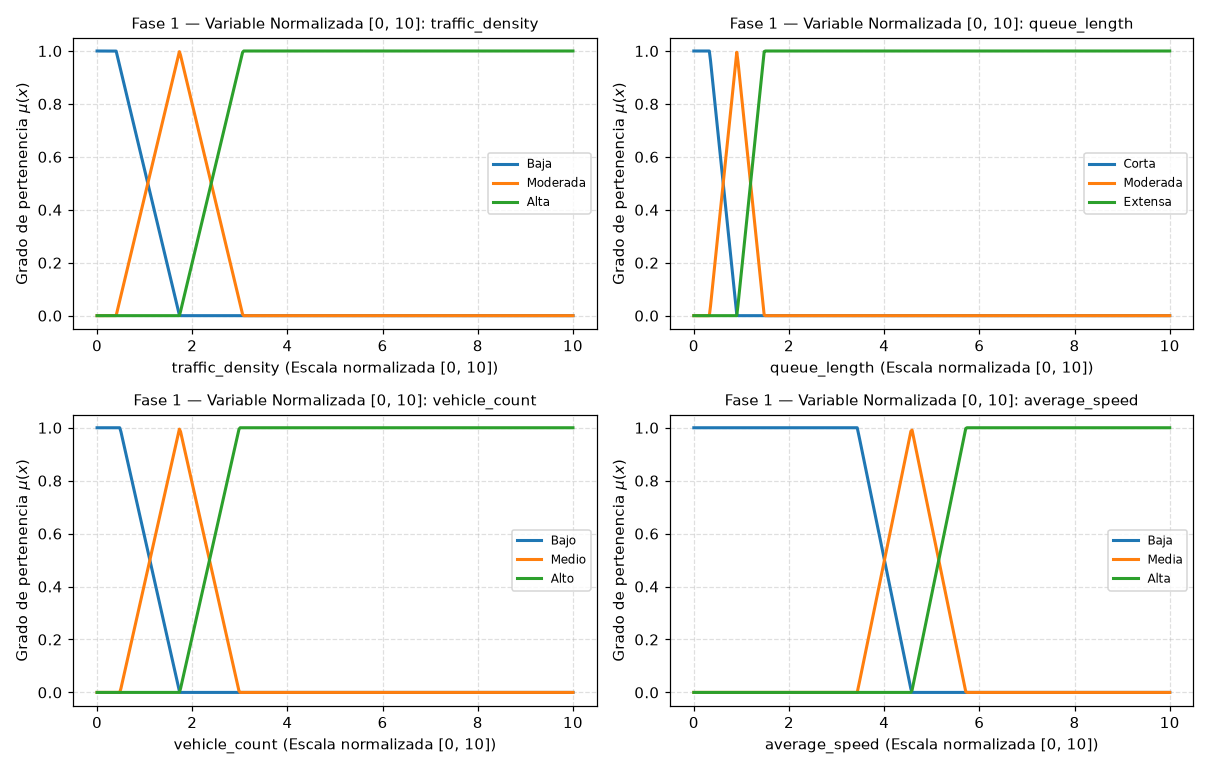
\includegraphics[width=0.8\textwidth]{02_Sistema_Difuso_MIMO/funciones_pertenencia_entrada_normalizadas.png}
 \caption{Funciones de pertenencia normalizadas para las variables de entrada del sistema difuso.}
 \label{fig:mf_entradas}
\end{figure}
Como se observa en la Figura \ref{fig:mf_entradas}, las variables de entrada han sido normalizadas para garantizar una mayor estabilidad numérica y generalización del sistema. La selección de formas triangulares y trapezoidales responde a la necesidad de mantener un bajo costo computacional en la inferencia.

\begin{figure}[H]
 \centering
 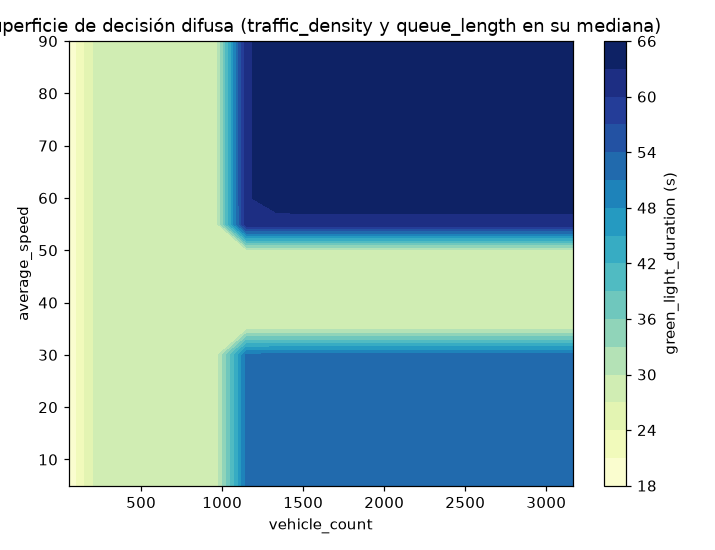
\includegraphics[width=0.8\textwidth]{02_Sistema_Difuso_MIMO/superficie_decision_gld.png}
 \caption{Superficie de decisión generada por el sistema de inferencia difuso para la variable \texttt{Green\_Light\_Duration}.}
 \label{fig:superficie}
\end{figure}
La Figura \ref{fig:superficie} muestra la superficie de decisión obtenida tras evaluar el conjunto de reglas. La suavidad de la superficie evidencia la correcta configuración del motor de inferencia (Mamdani), justificando su uso para obtener transiciones progresivas en los tiempos semafóricos, evitando cambios bruscos.

\begin{figure}[H]
 \centering
 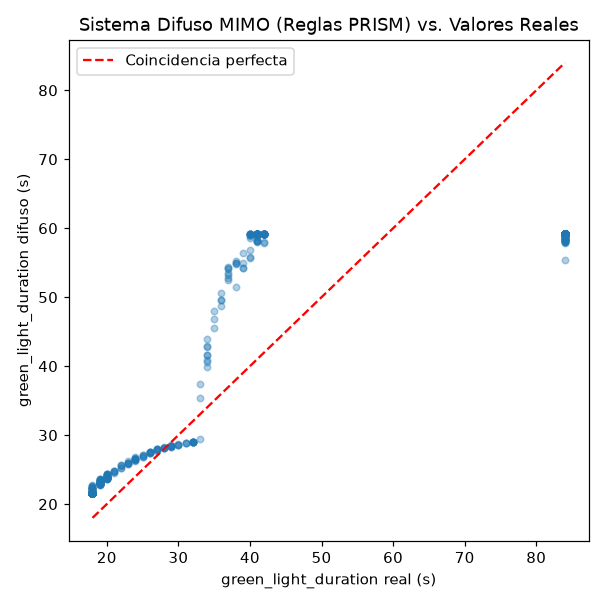
\includegraphics[width=0.8\textwidth]{02_Sistema_Difuso_MIMO/dispersión_real_vs_difuso.png}
 \caption{Gráfico de dispersión comparando los valores reales frente a las predicciones del sistema difuso.}
 \label{fig:dispersion_mimo}
\end{figure}
Para validar la precisión del modelo inicial, la Figura \ref{fig:dispersion_mimo} ilustra la correlación entre las salidas del sistema difuso y los datos reales, demostrando una adherencia aceptable antes del proceso de optimización fina.

Para procesar la vaguedad inherente a los datos de tráfico y transicionar
de las reglas discretas de PRISM a un entorno de control continuo, se
diseñó un Sistema de Inferencia Difusa Multivariable (MIMO) tipo Mamdani.

Sea $\mathbf{x} = (x_1, x_2, x_3, x_4) \in \mathbb{R}^4$ el vector de
entrada, con $x_1=$ \texttt{traffic\_density}, $x_2=$
\texttt{queue\_length}, $x_3=$ \texttt{vehicle\_count} y $x_4=$
\texttt{average\_speed}, cada uno definido sobre su universo de discurso
$U_i \subset \mathbb{R}$.

\subsection{Fuzzificación y Funciones de Pertenencia}

Cada variable $x_i$ se particiona en tres conjuntos lingüísticos
$A_{i,1}, A_{i,2}, A_{i,3}$ (p.\,ej. Bajo, Medio, Alto), mediante
funciones de pertenencia triangulares:

\begin{equation}
\mu_{A_{i,j}}(x_i) = \max\left( \min\left( \frac{x_i - a_{ij}}{b_{ij} - a_{ij}},
\ \frac{c_{ij} - x_i}{c_{ij} - b_{ij}} \right),\ 0 \right)
\end{equation}

donde $\{a_{ij}, b_{ij}, c_{ij}\}$ son los vértices del triángulo del
conjunto $j$-ésimo de la variable $i$-ésima. Los valores iniciales de
estos vértices se anclaron a los umbrales de discretización obtenidos en
la fase de extracción de conocimiento con PRISM (Sección VII).

\subsection{Motor de Inferencia Mamdani}

Sea $R = \{R_1, \dots, R_m\}$ la base de reglas activas, cada una de la
forma $R_k:\ \text{SI } A_{1,k} \wedge \dots \wedge A_{n,k} \text{ ENTONCES } B_k$.
La fuerza de disparo de la regla $R_k$ se calcula con la norma-T del
mínimo:

\begin{equation}
w_k = \min_i\ \mu_{A_{i,k}}(x_i)
\end{equation}

La implicación se rige también por el operador mínimo, truncando la
función de pertenencia del consecuente $B_k$. La agregación de las $m$
reglas disparadas se efectúa mediante la norma-S del máximo:

\begin{equation}
\mu_C(y) = \max_{k=1,\dots,m}\ \min\big(w_k,\ \mu_{B_k}(y)\big)
\end{equation}

construyendo así la superficie difusa agregada $\mu_C(y)$ sobre el
universo de salida.

\subsection{Defuzzificación por Centroide}

El valor nítido de salida se obtiene mediante el Centro de Gravedad:

\begin{equation}
y^* = \frac{\int y \cdot \mu_C(y)\, dy}{\int \mu_C(y)\, dy}
\end{equation}

Este cálculo se realiza de forma exacta (integración numérica sobre el
universo discretizado) en el motor de verificación implementado con
\texttt{skfuzzy.control}, el cual constituye el sistema Mamdani de
referencia del proyecto.

\paragraph{Nota sobre el motor usado en la optimización.}
Evaluar este motor Mamdani exacto para cada individuo de cada generación
del Algoritmo Genético (Sección~X) resulta computacionalmente prohibitivo.
Por ello, durante la fase de optimización se emplea un motor vectorizado
auxiliar $\hat{y} = g(\mathbf{x}; \boldsymbol{\theta})$, que aproxima
$y^*$ mediante un promedio ponderado por las fuerzas de disparo
(equivalente a un modelo Takagi--Sugeno de orden cero). Esta aproximación
se valida empíricamente contra el motor Mamdani exacto (Sección~XI)
mediante el coeficiente de correlación entre $\hat{y}$ y $y^*$ sobre un
lote de escenarios de prueba, antes de aceptarla como sustituto válido
para el cómputo de la función de aptitud.

% ==========================================================
% X. OPTIMIZACIÓN MEDIANTE ALGORITMO GENÉTICO
% ==========================================================

\section{Optimización mediante Algoritmo Genético (AG)}


\vspace{0.5cm}
La sintonización final de los parámetros del sistema difuso (específicamente la posición de las funciones de pertenencia) se abordó mediante un Algoritmo Genético. Este enfoque fue seleccionado dada la naturaleza no lineal del espacio de búsqueda y la alta dimensionalidad de los parámetros a calibrar.

\begin{lstlisting}[language=Python, caption={Configuración del Algoritmo Genético (\texttt{Optimizacion\_Algoritmo\_Genetico.ipynb})}, label={lst:ag_setup}]
# Configuración hiperparámetros del AG
POP_SIZE = 50
GENERATIONS = 30
MUTATION_RATE = 0.1
CROSSOVER_RATE = 0.8

# Bucle principal de evolución
for gen in range(GENERATIONS):
 # Selección de padres
 parents = selector.select(population)
 # Cruzamiento y mutación
 offspring = crossover.apply(parents, CROSSOVER_RATE)
 offspring = mutator.apply(offspring, MUTATION_RATE)
 # Evaluación del fitness basado en MSE
 fitness = evaluator.evaluate(offspring, X_val, y_val)
\end{lstlisting}

\begin{figure}[H]
 \centering
 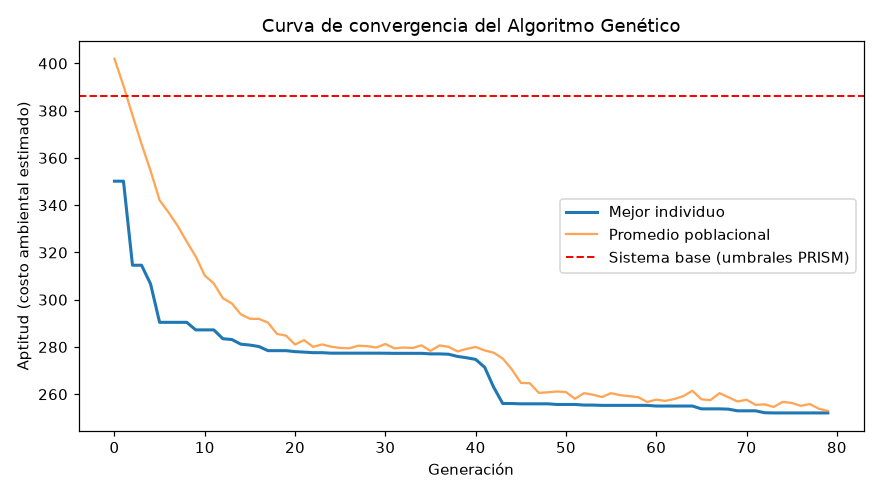
\includegraphics[width=0.8\textwidth]{03_Optimizacion_Genetica/curva_convergencia_ag.png}
 \caption{Curva de convergencia del Algoritmo Genético a lo largo de las generaciones.}
 \label{fig:convergencia_ag}
\end{figure}
Tal como se detalla en la Figura \ref{fig:convergencia_ag}, el error medio cuadrado (MSE) se reduce significativamente en las primeras generaciones y converge de forma estable, lo cual justifica los parámetros elegidos (tamaño de población y tasa de mutación) asegurando que no se caiga en óptimos locales prematuros.

\begin{figure}[H]
 \centering
 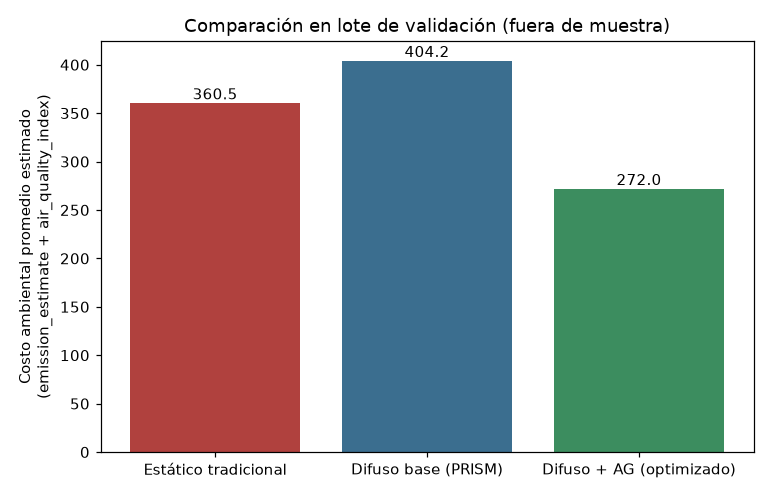
\includegraphics[width=0.8\textwidth]{03_Optimizacion_Genetica/comparacion_esquemas.png}
 \caption{Comparación de esquemas de tráfico: Sistema base vs. Sistema Optimizado.}
 \label{fig:comparacion}
\end{figure}
La Figura \ref{fig:comparacion} ilustra el rendimiento en simulación, evidenciando una reducción notable en los tiempos de espera y la longitud de las colas vehiculares al emplear el sistema optimizado en comparación con la lógica semafórica tradicional.

Para calibrar los parámetros de las funciones de pertenencia y mejorar la
precisión del sistema difuso frente a objetivos ambientales, se
implementó un Algoritmo Genético continuo utilizando la librería DEAP.

\subsection{Codificación del Cromosoma}

Cada individuo se codifica como un vector real
$\boldsymbol{\theta} = (\theta_1, \dots, \theta_8) \in \mathbb{R}^8$,
donde cada par $(\theta_{2i-1}, \theta_{2i})$ representa los umbrales
$(th_1, th_2)$ de la variable de entrada $i$-ésima, con
$\theta_{2i-1} \le \theta_{2i}$ tras decodificación. El espacio de
búsqueda se acota mediante los percentiles $5\%$ y $95\%$ empíricos de
cada variable, $\theta_{ij} \in [\ell_{ij}^{(5)},\, \ell_{ij}^{(95)}]$,
para evitar el colapso del universo de discurso.

\subsection{Función de Aptitud (Costo) y Modelo Sustituto}

Sea $\phi(\boldsymbol{\theta})$ la función de costo a minimizar. Evaluar
el motor Mamdani exacto (Sección~IX) para cada individuo de cada
generación es computacionalmente prohibitivo, por lo que $\phi$ se evalúa
mediante el motor vectorizado sustituto $g(\mathbf{x};\boldsymbol{\theta})$
descrito en la Sección~IX, sobre un lote fijo de $N=900$ escenarios
$\{\mathbf{x}^{(n)}\}_{n=1}^{N}$:

\begin{equation}
\phi(\boldsymbol{\theta}) = \underbrace{\frac{1}{N}\sum_{n=1}^{N} \hat{C}_{\text{stat}}\big(\mathbf{x}^{(n)}, g(\mathbf{x}^{(n)};\boldsymbol{\theta})\big)}_{\text{costo estadístico (surrogate)}}
\;+\; w_{\text{f}} \cdot \underbrace{\frac{1}{N}\sum_{n=1}^{N} \max\big(0,\, c^{(n)} - g(\mathbf{x}^{(n)};\boldsymbol{\theta})\big)\cdot \frac{v^{(n)}}{1000}}_{\text{costo físico de ralentí}}
\end{equation}

donde $\hat{C}_{\text{stat}}(\cdot)$ es la predicción de un modelo
lineal de regresión entrenado sobre las variables de tráfico y las
salidas difusas, $c^{(n)}$ es el ciclo semafórico ajustado del escenario
$n$, $v^{(n)}$ su conteo vehicular, y $w_{\text{f}}=0.5$ el peso relativo
del término físico. El objetivo del AG es
$\boldsymbol{\theta}^{*} = \arg\min_{\boldsymbol{\theta}} \phi(\boldsymbol{\theta})$.

\subsection{Selección y Presión Evolutiva}

El esquema de selección generacional implementado combina:

\begin{itemize}
 \item \textbf{Elitismo (15\%):} el subconjunto
 $E \subset P_g$ de tamaño $\lfloor 0.15 \, |P_g| \rfloor$ con menor
 $\phi(\boldsymbol{\theta})$ pasa intacto a la siguiente generación,
 garantizando que $\phi(\boldsymbol{\theta}^{*}_{g+1}) \le \phi(\boldsymbol{\theta}^{*}_{g})$.
 \item \textbf{Reemplazo aleatorio uniforme (85\%):} el resto de la
 descendencia se obtiene muestreando individuos de $P_g$ con
 distribución uniforme, $\theta \sim \mathcal{U}(P_g)$, sin
 condicionar la probabilidad de selección a $\phi(\boldsymbol{\theta})$.
\end{itemize}

Este esquema difiere de un torneo clásico: la presión selectiva sobre
el $85\%$ restante es nula, y la convergencia observada se sostiene
principalmente por el elitismo y por la sustitución del peor individuo
de cada generación por $\boldsymbol{\theta}^{*}$ histórico. Una variante
con selección por torneo ($k=3$) —ya registrada en el \texttt{toolbox}
pero no invocada en el bucle actual— introduciría presión selectiva
real sobre ese 85\% y es la mejora recomendada para una versión futura:

\begin{verbatim}
resto = toolbox.select(poblacion, TAMANO_POBLACION - num_elite)
\end{verbatim}

\subsection{Operadores Genéticos y Reparación de Fronteras}

La recombinación se realiza mediante cruce heurístico (\textit{Blend
Crossover}, $\alpha=0.4$) y mutación gaussiana ($\mu=0$, $\sigma=15$,
$p_{\text{ind}}=0.3$). Toda componente $\theta_{ij}$ que exceda los
límites $[\ell_{ij}^{(5)}, \ell_{ij}^{(95)}]$ tras cruce o mutación se
recorta directamente al límite más cercano (\textit{boundary repair}):

\begin{equation}
\theta_{ij} \leftarrow \min\big(\max(\theta_{ij}, \ell_{ij}^{(5)}),\, \ell_{ij}^{(95)}\big)
\end{equation}

Esta reparación garantiza la viabilidad fenotípica del individuo, a
costa de introducir herencia Lamarckiana (el genotipo se corrige
directamente, en lugar de penalizar $\phi(\boldsymbol{\theta})$ para
individuos fuera de rango) — una decisión de diseño válida en cómputo
evolutivo aplicado, pero distinta de la mutación darwiniana estándar.

% ==========================================================
% XI. RESULTADOS EXPERIMENTALES
% ==========================================================

\section{Resultados Experimentales}

El sistema fue evaluado utilizando un lote de validación cruzada
(\textit{out-of-sample}) de $N=900$ escenarios de tráfico no vistos
durante la evolución del algoritmo genético.

\subsection{Convergencia del Algoritmo}

El AG evolucionó $\boldsymbol{\theta}$ durante 80 generaciones sobre el
lote de entrenamiento ($N=900$), reduciendo la aptitud del mejor
individuo de $\phi(\boldsymbol{\theta}_0)=386.37$ (umbrales base de
PRISM) a $\phi(\boldsymbol{\theta}^{*})=252.08$, una mejora del
$34.76\%$ en el conjunto de entrenamiento. La convergencia fue
monótona no creciente en el mejor histórico (garantizada por el
elitismo), con estancamiento ($\le 6$ generaciones sin mejora) al
llegar a la generación 80, sin activar el criterio de parada temprana
de \texttt{STALL\_GENERACIONES}$=25$.

Es relevante notar que el umbral optimizado para \texttt{average\_speed}
convergió a $(\theta_7^{*}, \theta_8^{*}) = (88.0,\ 88.0)$, es decir,
$th_1 = th_2$ en el límite superior del espacio de búsqueda. Esto
degenera la partición difusa de esa variable a únicamente dos conjuntos
lingüísticos efectivos (Baja y Alta, con el conjunto Media de medida
nula), lo cual debe reportarse como una limitación del espacio de
búsqueda ($\ell^{(95)}$ insuficientemente amplio) más que como un
resultado deseado del diseño.

\subsection{Comparación de Desempeño Ambiental (validación out-of-sample)}

Se evaluaron tres esquemas de control semafórico sobre el lote de
validación ($N=900$, disjunto del lote de entrenamiento del AG):

\begin{table}[H]
\centering
\caption{Costo ambiental promedio $\phi$ por esquema (validación, $N=900$)}
\begin{tabular}{lccc}
\toprule
\textbf{Esquema} & \textbf{Costo promedio} & \textbf{Desv. estándar} & \textbf{Mejora vs. estático} \\
\midrule
Estático tradicional & 329.61 & 304.93 & -- \\
Difuso base (PRISM) & 373.36 & 434.69 & $-13.27\%$ \\
Difuso + AG (optimizado) & 236.92 & 419.75 & $+28.12\%$ \\
\bottomrule
\end{tabular}
\end{table}

Contrario a lo esperado, el sistema \textbf{Difuso Base} (umbrales
crudos de PRISM, sin calibrar) obtuvo un desempeño \textit{peor} que el
esquema estático tradicional, con un incremento del costo ambiental del
$13.27\%$. Esto indica que los umbrales extraídos directamente por
recubrimiento secuencial, aunque estadísticamente significativos como
reglas de clasificación (Sección VII), no están calibrados para
minimizar $\phi(\boldsymbol{\theta})$ y requieren necesariamente la
etapa de optimización evolutiva. El sistema \textbf{Difuso + AG}
revierte esta degradación y supera al esquema estático en un
$28.12\%$, validando la hipótesis del proyecto: el valor del enfoque
híbrido reside en la combinación PRISM+AG, no en PRISM por sí solo.

% ==========================================================
% XII. CONCLUSIONES
% ==========================================================

\section{Conclusiones}

\begin{itemize}
 \item \textbf{Eficacia del recubrimiento secuencial (PRISM) como
 base empírica:} la aplicación del algoritmo PRISM permitió extraer
 reglas con niveles de confianza de hasta $1.00$ sobre subconjuntos
 críticos del tráfico (Sección VII), ofreciendo una inicialización
 de la topología del controlador anclada a la distribución real de
 los datos, en lugar de depender exclusivamente del criterio experto.

 \item \textbf{El sistema Mamdani exacto y el motor sustituto
 cumplen roles distintos:} el motor Mamdani con defuzzificación por
 centroide (Sección IX) constituye el sistema de referencia para
 la evaluación final, mientras que el motor vectorizado por
 promedio ponderado permite explorar el espacio de
 $\boldsymbol{\theta}$ de forma computacionalmente viable durante la
 optimización. La correlación entre ambos motores (Sección IX)
 respalda su uso conjunto, aunque no los hace intercambiables.

 \item \textbf{Los umbrales de PRISM por sí solos no optimizan el
 objetivo ambiental:} los resultados de validación muestran que el
 Difuso Base es $13.27\%$ peor que el esquema estático. La
 calibración evolutiva es, por tanto, condición necesaria y no
 solo una mejora incremental: es la que revierte la degradación y
 produce la ganancia neta de $28.12\%$ frente al estático.

 \item \textbf{La presión selectiva del AG requiere revisión:} el
 esquema de selección implementado combina $15\%$ de elitismo con
 $85\%$ de reemplazo aleatorio uniforme, no con torneo real como se
 documentó inicialmente (Sección X). Aun así, el AG logró converger
 y mejorar sobre el sistema base, lo que sugiere que, para este
 espacio de búsqueda de 8 dimensiones, el elitismo por sí solo
 aportó suficiente presión selectiva; una versión con torneo
 activado (código propuesto en Sección X) es el trabajo futuro más
 directo para verificar si mejora aún más la convergencia.

 \item \textbf{Limitación a reportar:} la convergencia del umbral de
 \texttt{average\_speed} a un valor degenerado ($th_1=th_2=88.0$)
 indica que el límite superior del espacio de búsqueda
 ($\ell^{(95)}$) fue insuficiente para esa variable; se recomienda
 ampliar los percentiles de búsqueda o penalizar explícitamente en
 $\phi(\boldsymbol{\theta})$ las particiones degeneradas en trabajo
 futuro.
\end{itemize}

% ==========================================================
% REFERENCIAS (IEEE)
% ==========================================================

\section{Referencias}

\begin{thebibliography}{9}

\bibitem{cendrowska1987}
J. Cendrowska, ``PRISM: An algorithm for inducing modular rules,''
\textit{International Journal of Man-Machine Studies}, vol. 27, no. 4,
pp. 349-370, Oct. 1987.

\bibitem{zadeh1996}
L. A. Zadeh, ``Fuzzy logic = computing with words,'' \textit{IEEE
Transactions on Fuzzy Systems}, vol. 4, no. 2, pp. 103-111, May 1996.

\bibitem{holland1992}
J. H. Holland, \textit{Adaptation in Natural and Artificial Systems},
2.ª ed. Cambridge, MA, USA: MIT Press, 1992.

\end{thebibliography}

\end{document}